\documentclass[aspectratio=169
              ,usenames
              ,dvipsnames
              %uncomment to see notes
              %,handout
              ]{beamer}

\usetheme{metropolis}
%gets rid of bottom navigation bars
\definecolor{iicolor}{RGB}{232,150,70}
\setbeamercolor{frametitle}{bg=iicolor}
%\setbeamercolor{frametitle}{bg=white, fg=black}

\setbeamertemplate{footline}[frame number]{}

%gets rid of bottom navigation symbols
\setbeamertemplate{navigation symbols}{}

%gets rid of footer
%will override 'frame number' instruction above
%comment out to revert to previous/default definitions
\setbeamertemplate{footline}{}

%un-comment to see the notes
%\setbeameroption{show only notes} 

\usepackage{appendixnumberbeamer}
\usepackage{mathtools}
\usepackage{environ}
\usepackage{booktabs}
\usepackage{xcolor}
\usepackage{graphicx}
\usepackage{subcaption}
\captionsetup{compatibility=false}
\usepackage[scale=2]{ccicons}
\usepackage{hyperref}
\usepackage{pgfplots, pgfplotstable}
\usepackage{xparse}
\usepgfplotslibrary{dateplot}
\pgfplotsset{compat=1.12} % for better axis label placement

% Create a function for generating inverse normally distributed numbers using the Box–Muller transform
\pgfmathdeclarefunction{invgauss}{2}{%
  \pgfmathparse{sqrt(-2*ln(#1))*cos(deg(2*pi*#2))}%
}

\usetikzlibrary{decorations.text,graphs,graphs.standard,fadings,shapes.arrows,shadows}

\definecolor{mygray}{RGB}{208,208,208}
\definecolor{background}{RGB}{29,47,43}
\newcommand*{\mytextstyle}{\sffamily\small\bfseries\color{black!85}}
\usepackage{xspace}
\newcommand{\themename}{\textbf{\textsc{metropolis}}\xspace}
\newcommand\Wider[2][3em]{%
\makebox[\linewidth][c]{%
  \begin{minipage}{\dimexpr\textwidth+#1\relax}
  \raggedright#2
  \end{minipage}%
  }%
}

\title{{\bf Spark API Zoo}}
\date{}
\subtitle{An Overview}

\begin{document}

\maketitle
\begingroup
\Huge
\begin{frame}
\frametitle{Introduction}
\begin{center}
Hi, I'm Casey Stella!
\end{center}
\end{frame}
\endgroup

\frame{\frametitle{Low Level API - RDD}
  \begin{itemize}
    \item Primary API used in Spark 1.x\pause
    \item Does not presume structured data\pause
    \item Lowest level control\pause
      \begin{itemize}
        \item Basic functional-style distributed computing primitives\pause
        \item Ability to control data partition/placement\pause
        \item Ability to broadcast variables\pause
      \end{itemize}
  \end{itemize}
  RDDs are like C: maximum control with maximum opportunity to shoot yourself in the foot.
}

\frame{\frametitle{High Level API - DataFrame/Datasets}
  \begin{itemize}
    \item Primary API used in Spark 2.x\pause
    \item Table-like collection with well-defined rows and (nullable) columns and schemas.\pause
    \item These represent high level instructions which get converted into RDD transformations by a cost based optimizer.\pause
    \item DataFrame operations/capabilities are mostly unified between streaming and batch\pause
    \item Higher level control with more focus on relational primitives\pause
  \end{itemize}
  The attempt behind DataFrames is provides most of the flexibility of RDDs but hides some of the complexity.
}

\frame{\frametitle{High Level API - Datasets}
  Datasets are type-safe DataFrames.\pause
  \begin{itemize}
    \item There is a performance penalty for encoding/decoding to/from Row the custom data type.\pause
    \item This is useful when\pause
      \begin{itemize}
        \item You have a set of objects you want to share between spark/non-spark code.\pause
        \item You really, really want type-safety
      \end{itemize}
  \end{itemize}
}

\frame{\frametitle{High Level API - Spark SQL}
  Spark SQL is an alternative high level API which 
  \begin{itemize}
    \item Is ANSI SQL:2003 compliant\pause
    \item Integrates with the Hive metastore\pause
    \item Allows you to interact with the results of a query as a DataFrame\pause
  \end{itemize}
}

\frame{\frametitle{API Relationship}
\begin{center}
  \makebox[\textwidth]{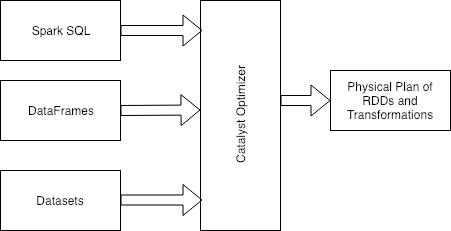
\includegraphics[scale=0.5]{images/api_overview.png}}
\end{center}
}



\frame{\frametitle{High Level API - Catalyst }
  Catalyst is a cost based optimizer which will map DataFrame operations to a physical plan.
  This provides some benefits:\pause
  \begin{itemize}
    \item A unified layer to apply optimizations which will affect DataFrame, SQL and Datasets\pause
    \item By providing an internal representation, many common transformations will operate outside of the host language.\pause
  \end{itemize}
  Key takeaway: Catalyst is a level of indirection that the community to centralize optimization work that will work across the logical APIs
}

\frame{\frametitle{Example: Off-Target Amplicon Detection}
Determining off-target amplicon matches are important parts of designing custom gene sequencing.
\begin{itemize}
  \item Compute amplicon matches
  \item Partition with overlap via a simple $k$ length strategy
  \item Determine which amplicon pairs are ``valid``
\end{itemize}
\makebox[\textwidth]{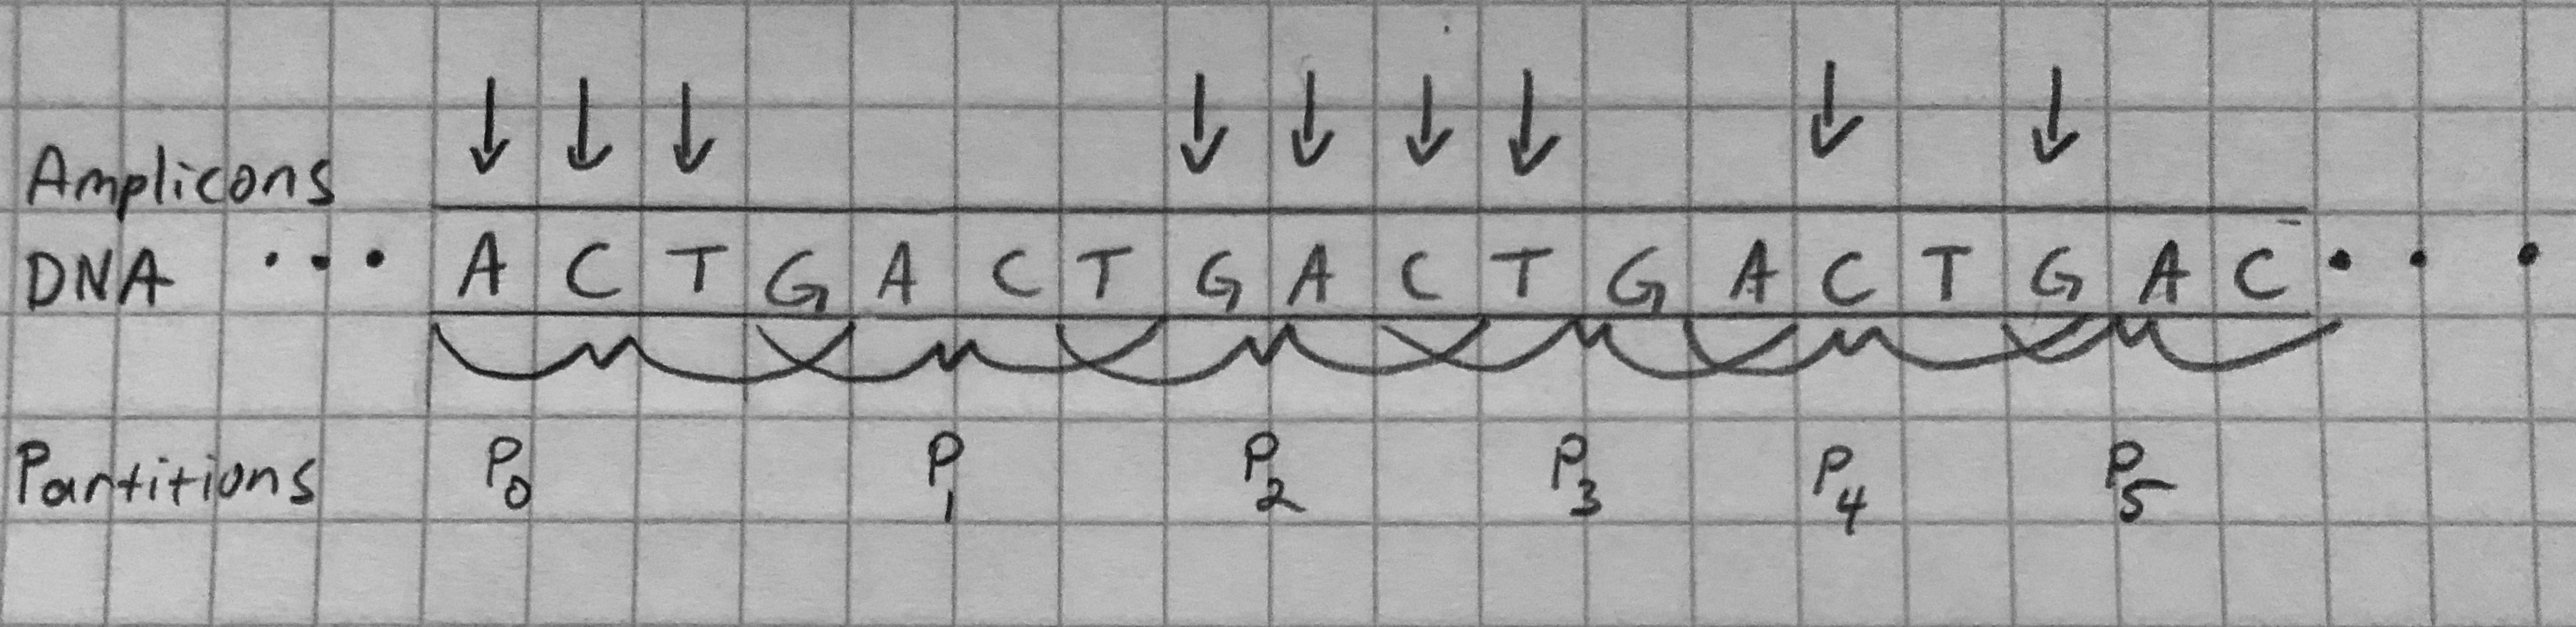
\includegraphics[scale=0.12]{images/dna_linear_partition.png}}
}

\frame{\frametitle{Example: Off-Target Amplicon Detection}
Problems
\begin{itemize}
  \item We're in a situation where we need to do a computationally complex operation with large constant per partition.
  \item Lots of mostly empty partitions!
\end{itemize}

\makebox[\textwidth]{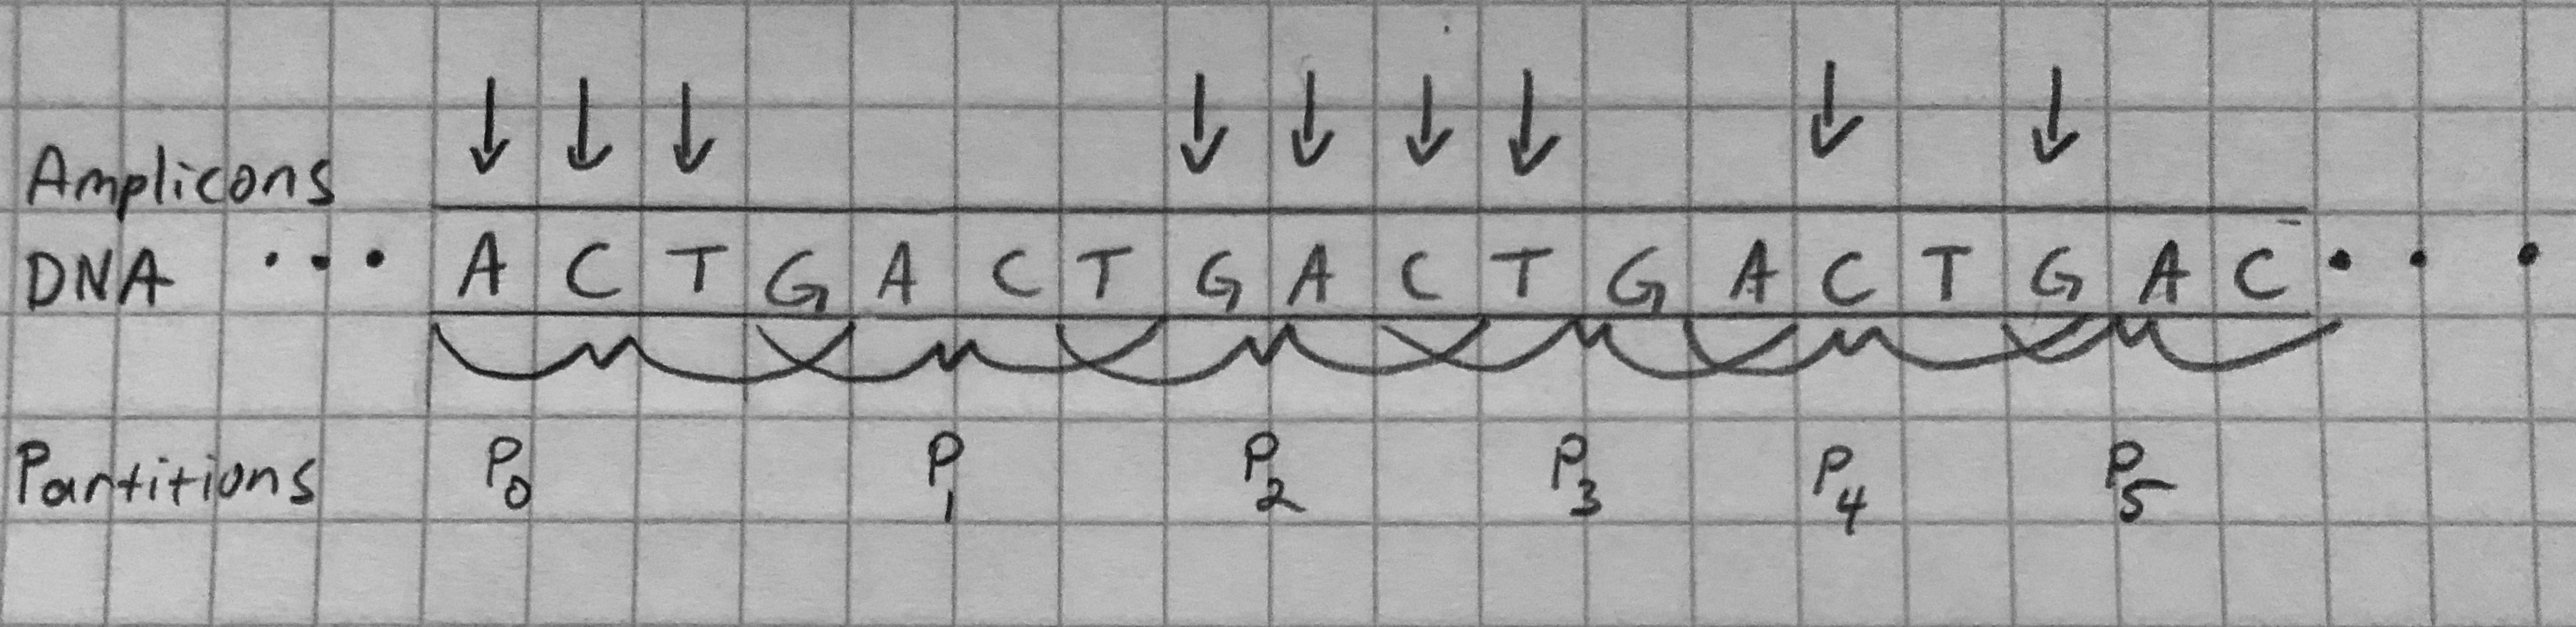
\includegraphics[scale=0.12]{images/dna_linear_partition.png}}
}

\frame{\frametitle{Example: Off-Target Amplicon Detection}
Percentile-based Partitioning
\begin{itemize}
  \item Compute amplicon matches
  \item Determine partition splits $\ni$ each partition contains an equal percent of matches
  \item Determine which amplicon pairs are ``valid`` with parallelism unit as the partition
\end{itemize}
\begin{center}
  \makebox[\textwidth]{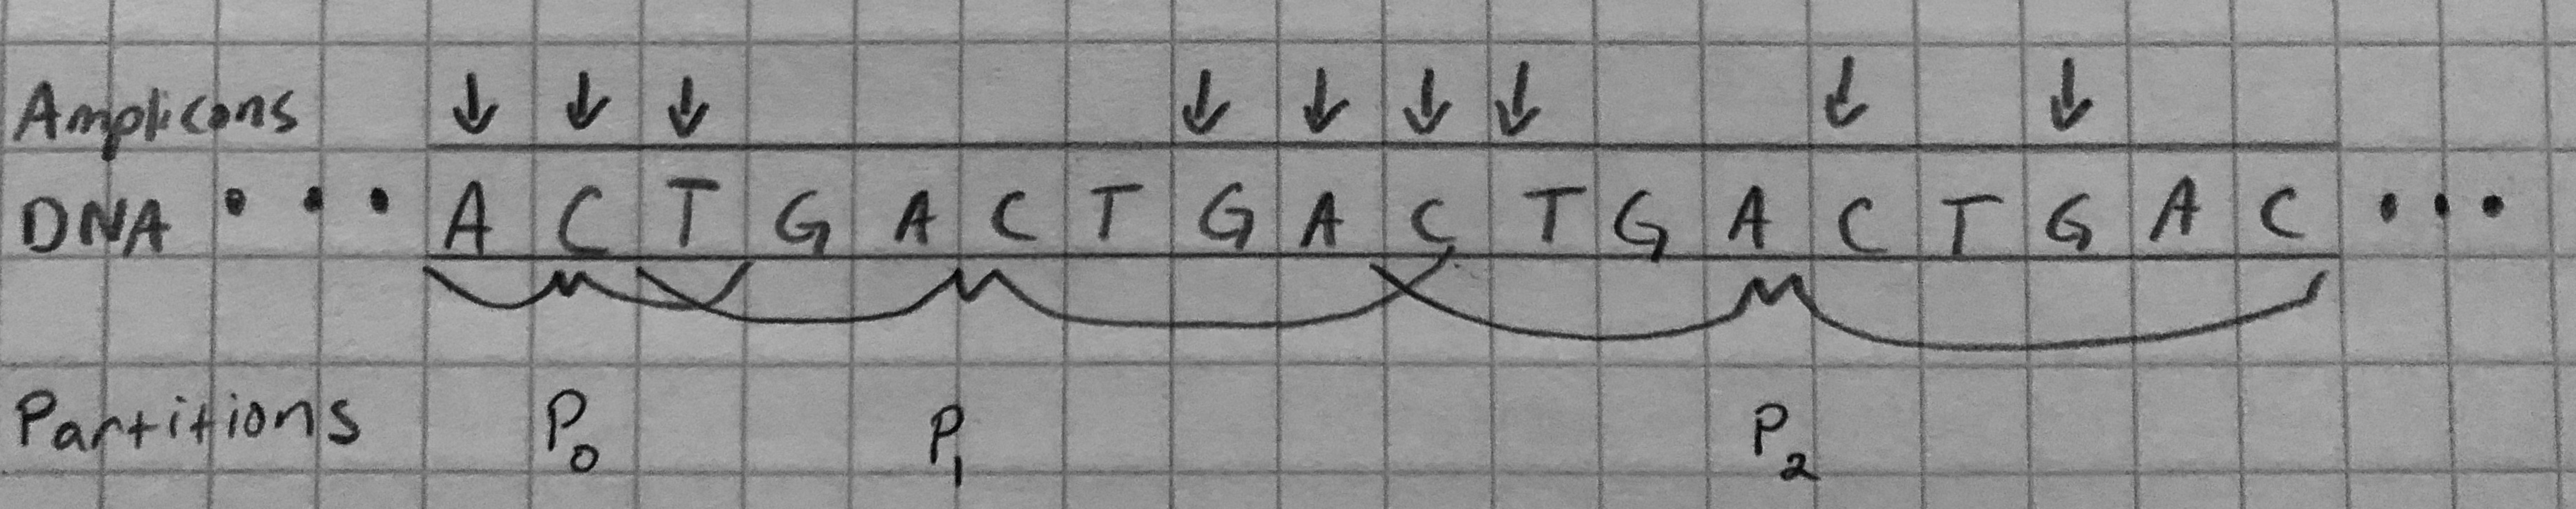
\includegraphics[scale=0.12]{images/dna_percentage_partition.png}}
\end{center}
}

\frame{\frametitle{Some Advice}
  \begin{itemize}
    \item Try to use dataframes and catalyst expressions as much as you can (expecially if working in a non-JVM language).\pause
    \item Don't be afraid to move up and down the stack of complexity as needed.\pause
    \item Using non-JVM languages requires care and understanding of data serialization costs.\pause
      \begin{itemize}
        \item It may be a winning strategy to implement common custom UDFs in a JVM language and use them.\pause
      \end{itemize}
    \item Mind memory and monitor garbage collection.
  \end{itemize}
}

\frame{\frametitle{Questions}
Thanks for your attention!  Questions? 
\begin{itemize}
\item This talk available on my github presentation page.\footnote{http://github.com/cestella/presentations/}
\item Find me at http://caseystella.com 
\item Twitter handle: @casey\_stella 
\end{itemize}
}

\end{document}
